\input{header.texinc}

\usepackage{nameref}
\usepackage{xr}
\externaldocument{appendix}
\newcommand{\fileref}[1]{\texttt{\nameref*{#1}} (appendix page~\pageref*{#1})}
\newcommand{\coderef}[1]{(appendix page~\pageref*{#1})}
\newcommand{\codenref}[1]{\texttt{#1} (appendix page~\pageref*{#1})}

\usepackage[]{tikz}
\usetikzlibrary{arrows.meta, positioning}

\title{Criterion C: Development}

\begin{document}
\maketitle

\renewcommand{\contentsname}{List of Techniques}
\tableofcontents

\section{Microsoft Entra ID Authentication}

User will need to be authenticated to use this system. Only teachers from the CCA department and students in the high school should be able to sign in to the system; therefore, I would like to integrate this with the school's existing authentication infrastructure, instead of using a separate accounts system. I could use either of the following methods:

\begin{enumerate}
	\item \label{method-entra} My system could redirect users to use Microsoft Entra ID Authentication via OpenID Connect.
	\item \label{method-powerschool} My system could accept users' usernames and passwords, and send them to PowerSchool and check if their credentials could be used to successfully log in.
\end{enumerate}

Although it is possible to store passwords securely with password-based key derivation algorithms such as Argon2 \parencite{argon2}, method~\ref{method-powerschool} still requires my sever to have ephemeral access to the user's school password in plain text form in memory, which is a security liability. It is also relatively difficult to store sensitive data correctly in memory, as that would involve, for example locking pages out of swap and overwriting relevant memory regions with random data, which is relatively difficult in Go.

Instead, I read the Microsoft Entra ID's OpenID Connect protocol reference \parencite{ms-oidc} and implemented it in \fileref{endpoint_auth.go}. \codenref{generateAuthorizationURL} generates an authorization URL for Microsoft Entra ID that the user is expected to visit; when the user finishes authentication on the Microsoft login form and consents to the application reading basic user information, their browser sends a POST request that is handled by \codenref{handleAuth} with an authorization token containing user data, signed by Microsoft. We check the validity of the signature and insert the user data (name, department, student ID, Microsoft Entra object UUID, etc) into the database while giving them a session cookie. From now on, we may authenticate the user's requests with their session cookie.

\begin{figure}
	\centering
	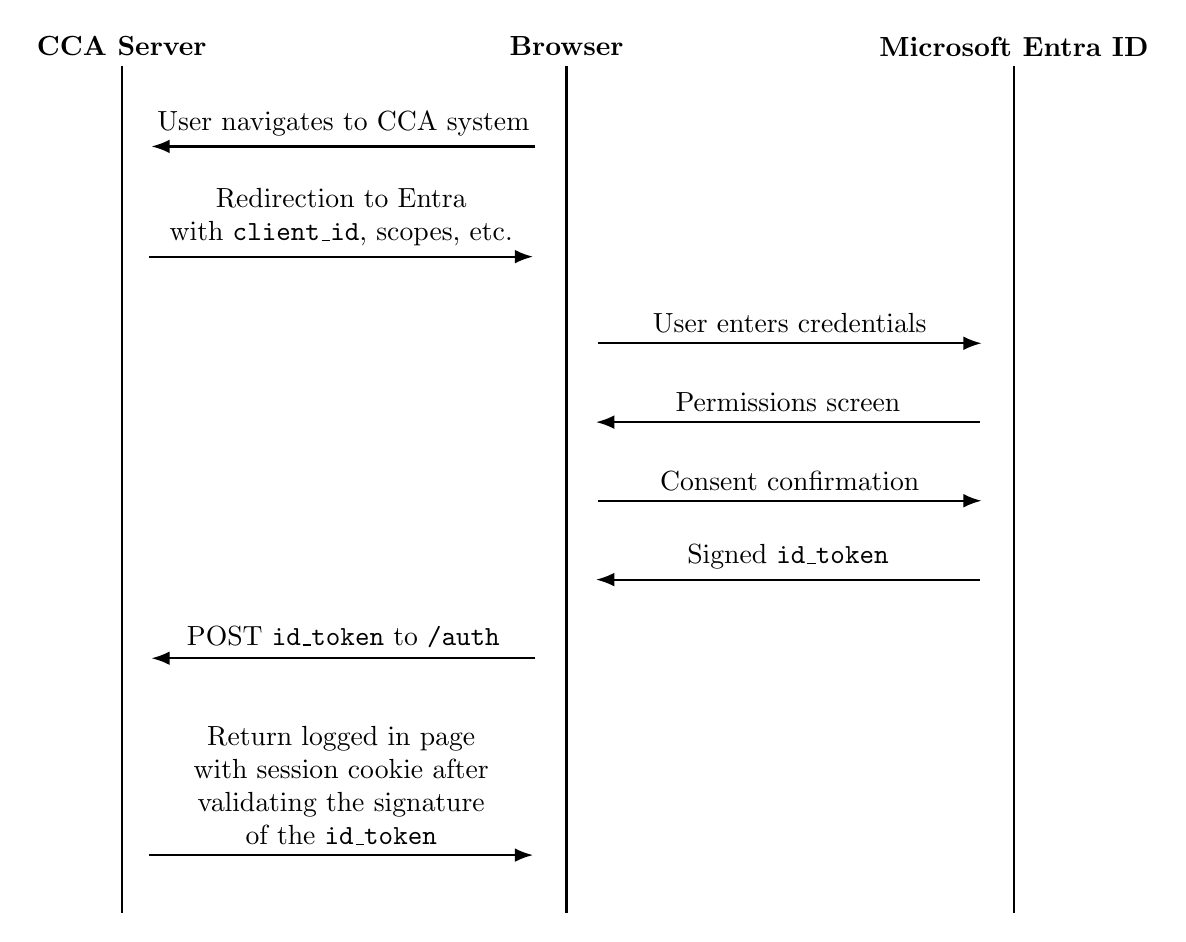
\begin{tikzpicture}[
		font=\normalsize,
		node distance=1cm and 2cm,
		>=Latex, 
		auto,
		every node/.style={align=center},
		sequence/.style={draw, thick},
		dashed sequence/.style={sequence, dashed},
		participant/.style={font=\bfseries},
		every arrow/.append style={thick},
		line/.style={draw, thick, ->}
	]
		\node[participant] (webserver) {CCA Server};
		\node[participant, right=of webserver, xshift=1.6cm] (browser) {Browser};
		\node[participant, right=of browser, xshift=1cm] (aad) {Microsoft Entra ID};
		
		\draw[sequence] (webserver) -- ++(0, -11);
		\draw[sequence] (browser) -- ++(0, -11);
		\draw[sequence] (aad) -- ++(0, -11);
	
		\node[below left= 0.9 and -0.7 of browser] (browser one) {};
		\draw[line] (browser one) -- ++(-5, 0) node[midway, above] {User navigates to CCA system};
		
		\node[below right= 2.3 and -1.1 of webserver] (webserver two) {};
		\draw[line] (webserver two) -- ++(5, 0) node[midway, above] {Redirection to Entra\\with \texttt{client\_id}, scopes, etc.};
		
		\node[below right= 3.4 and -0.7 of browser] (browser three) {};
		\draw[line] (browser three) -- ++(5, 0) node[midway, above] {User enters credentials};
		
		\node[below left= 4.4 and -1.65 of aad] (entra four) {};
		\draw[line] (entra four) -- ++(-5, 0) node[midway, above] {Permissions screen};
		
		\node[below right= 5.4 and -0.7 of browser] (browser five) {};
		\draw[line] (browser five) -- ++(5, 0) node[midway, above] {Consent confirmation};
		
		\node[below left= 6.4 and -1.65 of aad] (entra six) {};
		\draw[line] (entra six) -- ++(-5, 0) node[midway, above] {Signed \texttt{id\_token}};
		
		\node[below left= 7.4 and -0.7 of browser] (browser seven) {};
		\draw[line] (browser seven) -- ++(-5, 0) node[midway, above] {POST \texttt{id\_token} to \texttt{/auth}};
		
		\node[below right= 9.9 and -1.1 of webserver] (webserver eight) {};
		\draw[line] (webserver eight) -- ++(5, 0) node[midway, above] {Return logged in page\\with session cookie after\\validating the signature\\of the \texttt{id\_token}};
	\end{tikzpicture}
	\caption{OpenID Connect Sign-in Flow, modified from \textcite{ms-oidc}}
\end{figure}

\printbibliography

\end{document}
